\documentclass[11pt,a4paper]{article}

% ── Packages ──────────────────────────────────────────────────────────────────
\usepackage[utf8]{inputenc}
\usepackage[T1]{fontenc}
\usepackage{amsmath,amssymb,amsfonts}
\usepackage{physics}        % \braket, \bra, \ket, \expval
\usepackage{graphicx}
\usepackage[colorlinks=true,linkcolor=blue,citecolor=blue,urlcolor=blue]{hyperref}
\usepackage{listings}
\usepackage{geometry}
\usepackage{booktabs}
\usepackage{caption}
\usepackage{float}

\geometry{margin=1in}

\lstset{
  basicstyle=\ttfamily\footnotesize,
  keywordstyle=\color{blue},
  commentstyle=\color{gray},
  frame=single,
  breaklines=true
}

% ── Title ─────────────────────────────────────────────────────────────────────
\title{QAOA Energy Landscape Explorer:\\
  A Complete Mathematical Walkthrough\\
  for MaxCut on the 4-Node Cycle Graph}
\author{Generated Report}
\date{\today}

% ══════════════════════════════════════════════════════════════════════════════
\begin{document}
\maketitle
\tableofcontents
\newpage

% ══════════════════════════════════════════════════════════════════════════════
\section{Introduction}\label{sec:introduction}

The Quantum Approximate Optimization Algorithm (QAOA), introduced by Farhi,
Goldstone, and Gutmann~\cite{farhi2014}, is a hybrid quantum-classical
algorithm designed for combinatorial optimization on near-term quantum
hardware.  QAOA alternates between a \emph{cost unitary} that encodes the
objective function and a \emph{mixer unitary} that explores the solution space,
producing a parametrized quantum state whose expectation value approximates the
optimal cost.

This report presents a complete, self-contained mathematical walkthrough of the
QAOA energy landscape for the \textbf{MaxCut problem on the 4-node cycle graph
$C_4$}, at circuit depth $p=1$.  We proceed from the graph definition through
the Ising Hamiltonian, circuit construction, energy landscape analysis,
classical optimization, and finally noise modelling with zero-noise
extrapolation (ZNE) error mitigation.  Every derivation step is shown
explicitly so the reader can reproduce the results from first principles.

% ══════════════════════════════════════════════════════════════════════════════
\section{Problem Formulation}\label{sec:problem}

\subsection{The MaxCut Problem}

Given an undirected graph $G=(V,E)$ with edge weights $w_{ij}>0$, the
\textbf{MaxCut} problem asks for a partition of $V$ into two disjoint subsets
$S$ and $\bar{S}$ that maximises the total weight of edges crossing the
partition:
\begin{equation}\label{eq:maxcut-obj}
  \text{MaxCut}(G) \;=\; \max_{S \subseteq V}\; \sum_{(i,j)\in E} w_{ij}\,
    \bigl[\, i\in S,\; j\in\bar{S} \;\text{or}\; j\in S,\; i\in\bar{S}\,\bigr].
\end{equation}
Assigning Ising spin variables $z_i \in \{+1,-1\}$ to each vertex (with $z_i =
+1$ if $i\in S$ and $z_i = -1$ if $i\in\bar{S}$), the cost function becomes:
\begin{equation}\label{eq:cost-ising}
  C(\mathbf{z}) \;=\; \sum_{(i,j)\in E} w_{ij}\,\frac{1 - z_i z_j}{2}.
\end{equation}
A cut edge contributes $1$ (since $z_i z_j = -1$) while an uncut edge
contributes $0$ (since $z_i z_j = +1$).

\subsection{The 4-Node Cycle Graph $C_4$}

We consider the cycle graph on four vertices:
\begin{align}
  V &= \{0,\,1,\,2,\,3\}, \\
  E &= \{(0,1),\;(1,2),\;(2,3),\;(3,0)\}, \\
  w_{ij} &= 1 \quad \forall\; (i,j)\in E.
\end{align}
The cost function for $C_4$ is therefore:
\begin{equation}\label{eq:cost-c4}
  C(\mathbf{z}) \;=\; \frac{1-z_0 z_1}{2} + \frac{1-z_1 z_2}{2}
                     + \frac{1-z_2 z_3}{2} + \frac{1-z_3 z_0}{2}.
\end{equation}
Enumerating all $2^4=16$ bitstrings, the maximum cut is:
\begin{equation}
  C_{\max} = 4, \qquad \text{achieved by } \mathbf{z}^* \in \{0101,\; 1010\},
\end{equation}
where we use the binary encoding $z_i = (-1)^{x_i}$ with $x_i\in\{0,1\}$.
The minimum cut is $C_{\min}=0$, attained by $\{0000,\;1111\}$.

\begin{figure}[H]
  \centering
  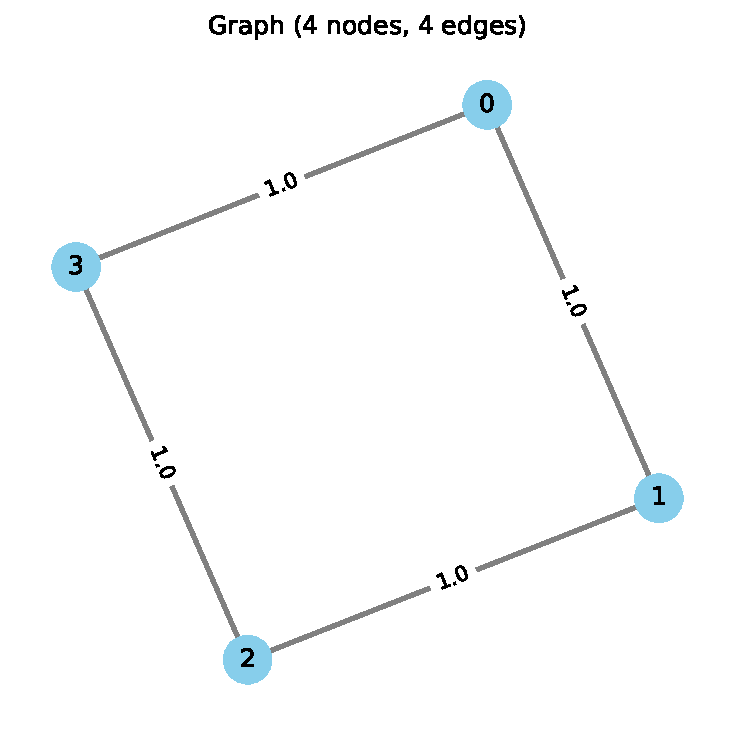
\includegraphics[width=0.45\textwidth]{report1_scripts/output/graph.pdf}
  \caption{The 4-node cycle graph $C_4$ with unit edge weights.}
  \label{fig:graph}
\end{figure}

% ══════════════════════════════════════════════════════════════════════════════
\section{Ising Hamiltonian}\label{sec:hamiltonian}

\subsection{General Construction}

Promoting the classical spins $z_i$ to Pauli-$Z$ operators $Z_i$ acting on
qubit $i$, the cost Hamiltonian is:
\begin{equation}\label{eq:HC-general}
  H_C \;=\; \sum_{(i,j)\in E} \frac{w_{ij}}{2}\bigl(I - Z_i Z_j\bigr),
\end{equation}
where $I$ is the identity operator on the full $2^n$-dimensional Hilbert space.
By construction, $H_C$ is diagonal in the computational basis and its
eigenvalues are the cut values:
\begin{equation}
  H_C \ket{\mathbf{x}} = C(\mathbf{x})\,\ket{\mathbf{x}}.
\end{equation}

\subsection{Explicit Form for $C_4$}

Substituting the four edges of $C_4$ with $w_{ij}=1$:
\begin{equation}\label{eq:HC-c4}
  H_C \;=\; \frac{1}{2}\Bigl[
    (I - Z_0 Z_1) + (I - Z_1 Z_2) + (I - Z_2 Z_3) + (I - Z_3 Z_0)
  \Bigr].
\end{equation}
Collecting the identity terms ($4 \times \tfrac{1}{2} = 2$):
\begin{equation}\label{eq:HC-simplified}
  \boxed{H_C \;=\; 2I \;-\; \frac{1}{2}\bigl(
    Z_0 Z_1 + Z_1 Z_2 + Z_2 Z_3 + Z_3 Z_0
  \bigr).}
\end{equation}

\subsection{Eigenvalue Verification}

Since $H_C$ is diagonal in the computational basis, we verify selected
eigenvalues.  For a computational basis state $\ket{x_0 x_1 x_2 x_3}$, each
$Z_i$ has eigenvalue $(-1)^{x_i}$.

\begin{table}[H]
\centering
\caption{Eigenvalues of $H_C$ for selected basis states of $C_4$.}
\label{tab:eigenvalues}
\begin{tabular}{ccccccc}
\toprule
$\ket{x_0 x_1 x_2 x_3}$ & $Z_0Z_1$ & $Z_1Z_2$ & $Z_2Z_3$ & $Z_3Z_0$
  & $\sum Z_iZ_j$ & $C(\mathbf{x})$ \\
\midrule
$\ket{0000}$ & $+1$ & $+1$ & $+1$ & $+1$ & $+4$ & $0$ \\
$\ket{1111}$ & $+1$ & $+1$ & $+1$ & $+1$ & $+4$ & $0$ \\
$\ket{0001}$ & $+1$ & $+1$ & $-1$ & $-1$ & $0$ & $2$ \\
$\ket{0011}$ & $+1$ & $-1$ & $-1$ & $+1$ & $0$ & $2$ \\
$\ket{0101}$ & $-1$ & $-1$ & $-1$ & $-1$ & $-4$ & $4$ \\
$\ket{1010}$ & $-1$ & $-1$ & $-1$ & $-1$ & $-4$ & $4$ \\
\bottomrule
\end{tabular}
\end{table}

Using Eq.~\eqref{eq:HC-simplified}, $C(\mathbf{x}) = 2 - \frac{1}{2}\sum
Z_iZ_j$, which matches the expected cut values.  The maximum eigenvalue is
$C_{\max}=4$ for the alternating bitstrings $\ket{0101}$ and $\ket{1010}$,
confirming the classical result.

% ══════════════════════════════════════════════════════════════════════════════
\section{QAOA Circuit Construction}\label{sec:circuit}

\subsection{The QAOA Ansatz}

For depth $p=1$, the QAOA state is:
\begin{equation}\label{eq:qaoa-state}
  \ket{\psi(\gamma,\beta)} \;=\; U_B(\beta)\, U_C(\gamma)\, \ket{+}^{\otimes n},
\end{equation}
where $\ket{+}^{\otimes n} = H^{\otimes n}\ket{0}^{\otimes n} =
\frac{1}{2^{n/2}}\sum_{\mathbf{x}\in\{0,1\}^n}\ket{\mathbf{x}}$ is the
uniform superposition.

\subsection{Cost Unitary $U_C(\gamma)$}

The cost unitary is the time evolution under $H_C$:
\begin{equation}\label{eq:UC}
  U_C(\gamma) \;=\; e^{-i\gamma H_C}
  \;=\; \prod_{(i,j)\in E} e^{-i\gamma \frac{1}{2}(I - Z_i Z_j)}.
\end{equation}
The product form holds because all $Z_iZ_j$ terms commute (they are
simultaneously diagonal).  Expanding each factor:
\begin{equation}
  e^{-i\gamma \frac{1}{2}(I - Z_i Z_j)}
  \;=\; e^{-i\gamma/2}\, e^{i\gamma/2\, Z_i Z_j}.
\end{equation}
The global phase $e^{-i\gamma/2}$ per edge accumulates to $e^{-2i\gamma}$ for
the four edges of $C_4$, and can be dropped since it does not affect
expectation values.  The non-trivial part is:
\begin{equation}\label{eq:UC-gates}
  U_C(\gamma) \;\sim\; \prod_{(i,j)\in E} e^{i\gamma/2\, Z_i Z_j}.
\end{equation}

\subsection{Gate Decomposition: $\mathrm{IsingZZ}$ Gates}

Each two-qubit term $e^{i\gamma/2\, Z_iZ_j}$ is an $\mathrm{IsingZZ}$ (or
$R_{ZZ}$) gate.  In terms of CNOT and $R_Z$ gates:
\begin{equation}
  e^{i\theta\, Z_i Z_j} \;=\;
  \mathrm{CNOT}(i,j)\;\cdot\; R_Z(2\theta)_j \;\cdot\; \mathrm{CNOT}(i,j),
\end{equation}
where $R_Z(\phi) = e^{-i\phi Z/2}$.  For our circuit, $\theta = \gamma/2$, so
each edge contributes:
\begin{equation}
  \mathrm{CNOT}(i,j) \;\to\; R_Z(\gamma)_j \;\to\; \mathrm{CNOT}(i,j).
\end{equation}

\subsection{Mixer Unitary $U_B(\beta)$}

The mixer unitary applies single-qubit $X$-rotations:
\begin{equation}\label{eq:UB}
  U_B(\beta) \;=\; \prod_{i=0}^{n-1} e^{-i\beta X_i}
  \;=\; \prod_{i=0}^{n-1} R_X(2\beta)_i,
\end{equation}
where $R_X(\phi) = e^{-i\phi X/2}$.

\subsection{Circuit Diagram}

The complete $p=1$ QAOA circuit for $C_4$ consists of the following layers:

\begin{enumerate}
  \item \textbf{Initialization}: Apply $H$ (Hadamard) to all 4 qubits:
        $\ket{0}^{\otimes 4} \to \ket{+}^{\otimes 4}$.
  \item \textbf{Cost layer} $U_C(\gamma)$: Four $\mathrm{IsingZZ}(-\gamma)$
        gates, one per edge:
        \begin{itemize}
          \item $\mathrm{ZZ}(\gamma)$ on qubits $(0,1)$
          \item $\mathrm{ZZ}(\gamma)$ on qubits $(1,2)$
          \item $\mathrm{ZZ}(\gamma)$ on qubits $(2,3)$
          \item $\mathrm{ZZ}(\gamma)$ on qubits $(3,0)$
        \end{itemize}
  \item \textbf{Mixer layer} $U_B(\beta)$: Four $R_X(2\beta)$ gates, one per
        qubit.
  \item \textbf{Measurement}: Measure all qubits in the computational basis.
\end{enumerate}

% ══════════════════════════════════════════════════════════════════════════════
\section{Energy Landscape}\label{sec:landscape}

\subsection{Energy Function}

The QAOA energy (objective function) is the expectation value of $H_C$ in the
variational state:
\begin{equation}\label{eq:energy}
  E(\gamma,\beta) \;=\; \expval{H_C}{\psi(\gamma,\beta)}
  \;=\; \bra{+}^{\otimes n} U_C^\dagger(\gamma)\, U_B^\dagger(\beta)\,
        H_C\, U_B(\beta)\, U_C(\gamma) \ket{+}^{\otimes n}.
\end{equation}

\subsection{Periodicity}

For MaxCut on unweighted graphs, the energy landscape exhibits the following
periodicity:
\begin{itemize}
  \item $E(\gamma,\beta)$ is $\pi$-periodic in $\gamma$, since the cost
        unitary involves $e^{i\gamma Z_iZ_j}$ and $Z_iZ_j$ has eigenvalues
        $\pm 1$.
  \item $E(\gamma,\beta)$ is $\pi/2$-periodic in $\beta$ (for the standard
        transverse-field mixer on MaxCut), arising from the symmetry of the
        $R_X$ rotation and the $\mathbb{Z}_2$ symmetry of the cost function.
\end{itemize}
It therefore suffices to scan $\gamma \in [0,\pi]$ and $\beta \in [0,\pi/2]$.

\subsection{Analytical Expression for $p=1$}

For a $d$-regular graph with $n$ vertices and $m=|E|$ edges at $p=1$, the QAOA
energy has the closed-form expression (see~\cite{farhi2014,wang2018}):
\begin{equation}\label{eq:energy-analytic}
  E(\gamma,\beta) \;=\; \frac{m}{2} + \frac{1}{2}\sum_{(i,j)\in E}
    \Bigl\langle Z_i Z_j \Bigr\rangle_{\gamma,\beta},
\end{equation}
where each $\langle Z_iZ_j\rangle$ depends on the local subgraph around edge
$(i,j)$.  For the 2-regular cycle $C_4$:
\begin{equation}
  \langle Z_iZ_j \rangle \;=\; \frac{1}{2}\sin(4\beta)\sin(2\gamma)
  \bigl[\cos(2\gamma) + \cos^2(2\gamma)\bigr]
  - \frac{1}{2}\sin^2(2\beta)\bigl[1 - \cos^2(2\gamma)\bigr].
\end{equation}
By symmetry all four edges give the same contribution, so:
\begin{equation}
  E(\gamma,\beta) \;=\; 2 - 2\langle Z_iZ_j \rangle.
\end{equation}

\subsection{Landscape Visualisations}

\begin{figure}[H]
  \centering
  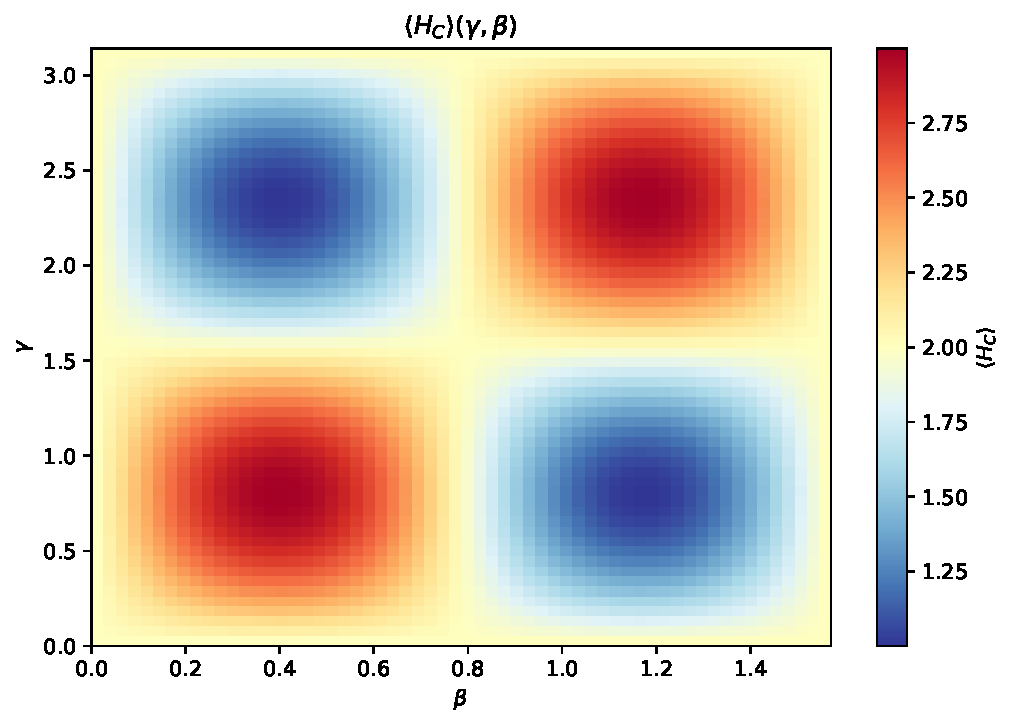
\includegraphics[width=0.75\textwidth]{report1_scripts/output/landscape_2d.pdf}
  \caption{2D heatmap of the QAOA energy $E(\gamma,\beta)$ for $C_4$ at $p=1$.
  The global maximum (brightest region) occurs near
  $(\gamma^*,\beta^*)\approx(\pi/4,\,5\pi/8)$.}
  \label{fig:landscape-2d}
\end{figure}

\begin{figure}[H]
  \centering
  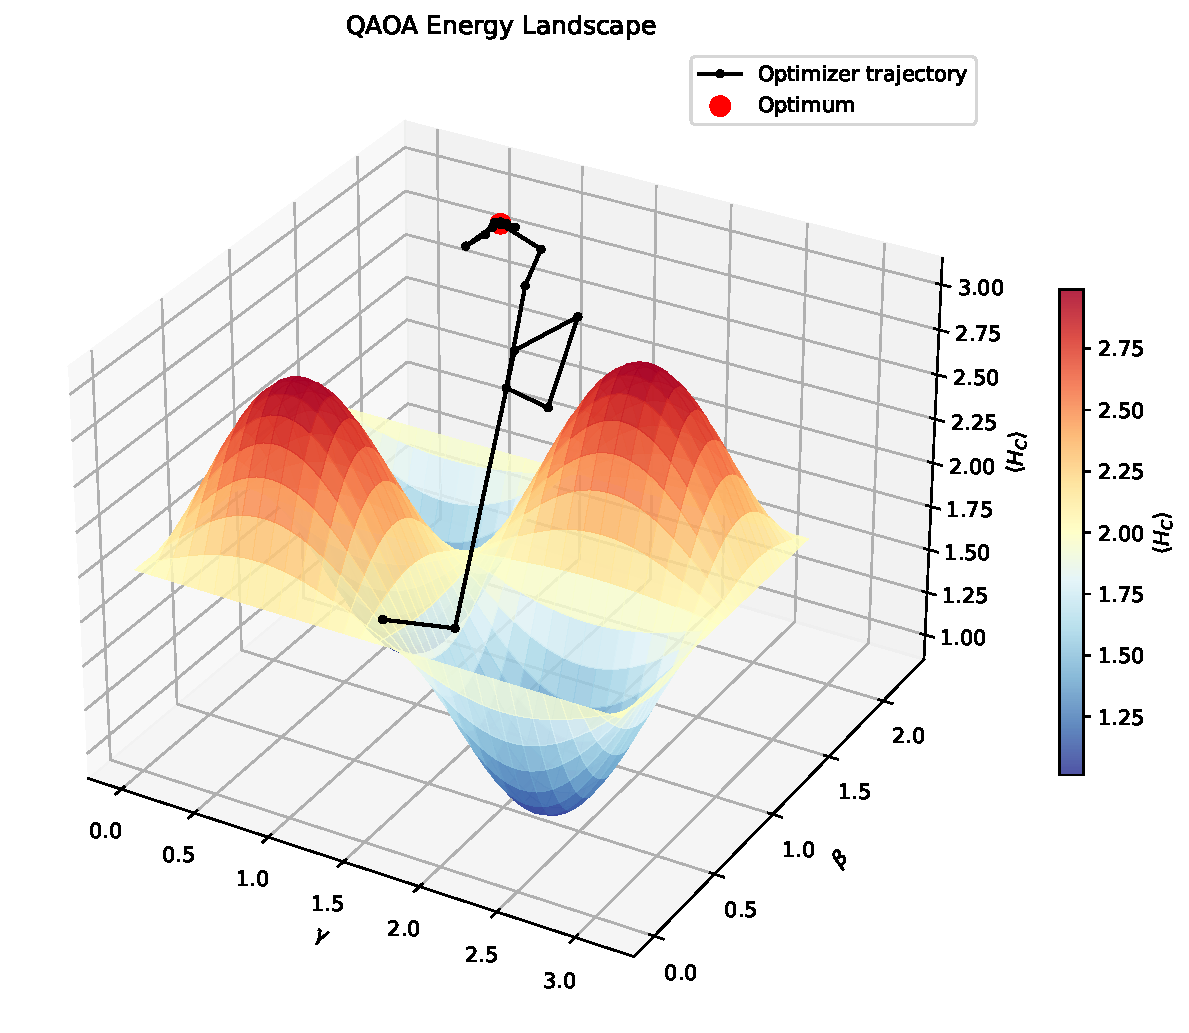
\includegraphics[width=0.75\textwidth]{report1_scripts/output/landscape_3d.pdf}
  \caption{3D surface plot of the QAOA energy landscape for $C_4$ at $p=1$.}
  \label{fig:landscape-3d}
\end{figure}

\begin{figure}[H]
  \centering
  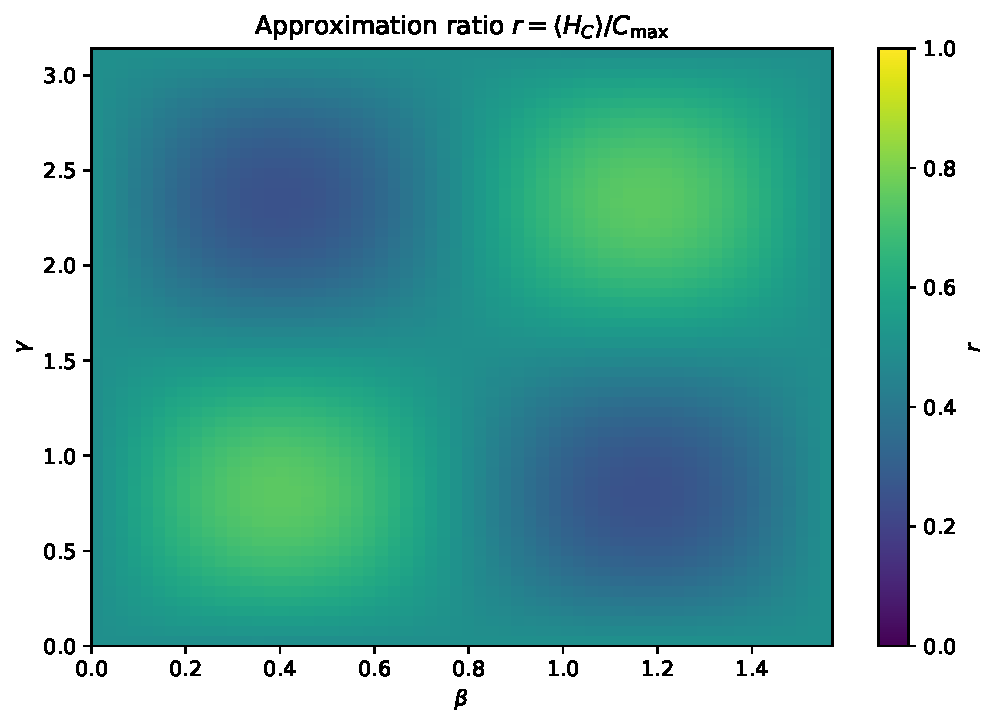
\includegraphics[width=0.75\textwidth]{report1_scripts/output/approx_ratio.pdf}
  \caption{Approximation ratio $r(\gamma,\beta) = E(\gamma,\beta)/C_{\max}$
  across the parameter space.  The maximum approximation ratio is $r=0.75$.}
  \label{fig:approx-ratio}
\end{figure}

\subsection{Observed Features}

Several features are evident in Figures~\ref{fig:landscape-2d}--\ref{fig:approx-ratio}:
\begin{itemize}
  \item \textbf{Global maximum}: The energy attains its maximum $E^*=3.0$ at
        $(\gamma^*,\beta^*) \approx (\pi/4,\; 5\pi/8)$, yielding an
        approximation ratio $r = 3/4 = 0.75$.
  \item \textbf{Symmetry}: The landscape is symmetric under
        $\beta \to \pi/2 - \beta$ (reflection about $\beta=\pi/4$) and
        exhibits the expected periodicity.
  \item \textbf{Multiple local extrema}: The landscape contains saddle points
        and local minima, illustrating why gradient-free optimizers or careful
        initialization are needed.
  \item \textbf{Smooth structure}: The landscape is smooth and differentiable,
        which is a consequence of the shallow ($p=1$) circuit and the small
        graph size.
\end{itemize}

% ══════════════════════════════════════════════════════════════════════════════
\section{Classical Optimization}\label{sec:optimization}

\subsection{Optimisation Problem}

The variational loop seeks to maximise the energy, or equivalently minimise its
negation:
\begin{equation}\label{eq:opt}
  (\gamma^*,\beta^*) \;=\; \arg\max_{\gamma,\beta}\, E(\gamma,\beta)
  \;=\; \arg\min_{\gamma,\beta}\, \bigl[-E(\gamma,\beta)\bigr].
\end{equation}

\subsection{COBYLA Optimizer}

We use the \textbf{Constrained Optimization BY Linear Approximations (COBYLA)}
algorithm~\cite{powell1994}, a gradient-free method that:
\begin{itemize}
  \item Constructs a linear approximation to the objective in a trust region.
  \item Updates the trust region radius (starting from \texttt{rhobeg}) at each
        iteration.
  \item Does not require gradient evaluations, making it suitable for noisy
        quantum objectives.
\end{itemize}

\subsection{Parameter-Shift Rule}

Although COBYLA is gradient-free, gradient-based optimizers can exploit the
\textbf{parameter-shift rule}.  For a parameter $\theta_i$ appearing in a gate
$e^{-i\theta_i G/2}$ where $G$ has eigenvalues $\pm 1$:
\begin{equation}\label{eq:param-shift}
  \frac{\partial E}{\partial \theta_i}
  \;=\; \frac{E(\theta_i + \pi/2) - E(\theta_i - \pi/2)}{2}.
\end{equation}
This provides exact (not finite-difference) gradients using only two circuit
evaluations per parameter, and is an alternative strategy for landscape
navigation.

\subsection{Convergence}

\begin{figure}[H]
  \centering
  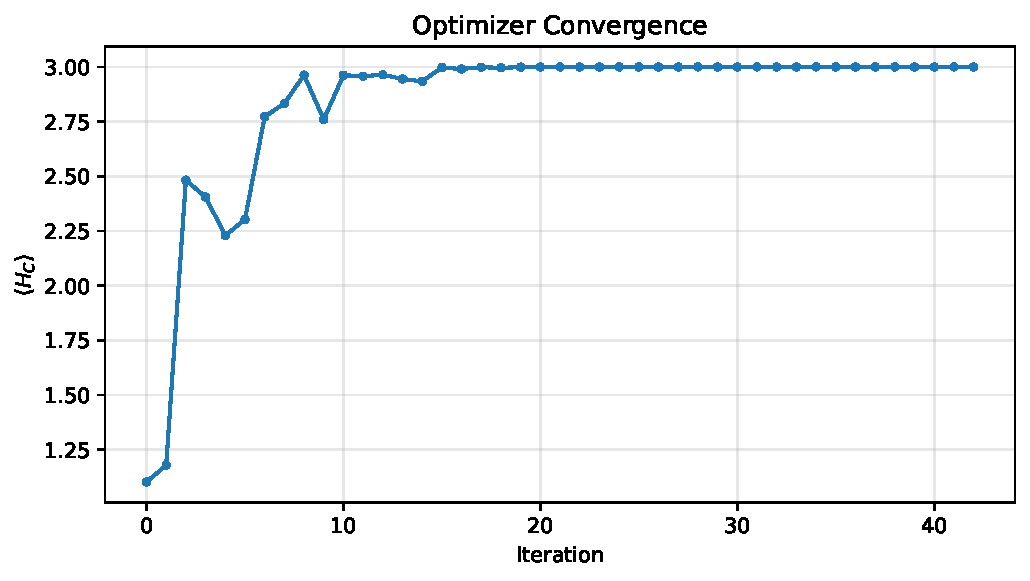
\includegraphics[width=0.75\textwidth]{report1_scripts/output/convergence.pdf}
  \caption{Convergence of the COBYLA optimizer.  The algorithm reaches the
  optimal energy $E^*=3.0$ within 43 function evaluations.}
  \label{fig:convergence}
\end{figure}

\subsection{Results}

The optimizer converged in \textbf{43 function evaluations} to:
\begin{align}
  \gamma^* &\approx \frac{\pi}{4} \approx 0.7854, \label{eq:gamma-star}\\
  \beta^*  &\approx \frac{5\pi}{8} \approx 1.9635, \label{eq:beta-star}\\
  E^*      &= 3.0, \label{eq:E-star}\\
  r^*      &= \frac{E^*}{C_{\max}} = \frac{3.0}{4.0} = 0.75. \label{eq:r-star}
\end{align}

\subsection{Discussion}

The theoretical maximum approximation ratio for $p=1$ QAOA on the cycle graph
$C_4$ is indeed $r=0.75$, consistent with the general result that depth-1 QAOA
on $2$-regular (cycle) graphs achieves:
\begin{equation}
  r_{p=1} \;=\; \frac{3}{4}
\end{equation}
for all cycle lengths $n\geq 4$.  This bound can be improved by increasing the
circuit depth $p$; for $p\to\infty$, QAOA recovers the exact solution
$r\to 1$.

% ══════════════════════════════════════════════════════════════════════════════
\section{Noise Effects and Error Mitigation}\label{sec:noise}

\subsection{Noise Model}

To simulate realistic near-term hardware, we apply a noise model consisting of
two channels:

\paragraph{Depolarizing channel.}
After each gate, a depolarizing channel with error probability $p_{\text{dep}}
= 0.01$ is applied:
\begin{equation}
  \mathcal{E}_{\text{dep}}(\rho) \;=\; (1 - p_{\text{dep}})\,\rho
  \;+\; \frac{p_{\text{dep}}}{2^k - 1}\sum_{P \neq I} P\,\rho\, P^\dagger,
\end{equation}
where the sum runs over all $k$-qubit Pauli operators (excluding identity) and
$k$ is the number of qubits the gate acts on.

\paragraph{Thermal relaxation.}
We model decoherence with relaxation times:
\begin{align}
  T_1 &= 50\;\mu\text{s}, &
  T_2 &= 70\;\mu\text{s},
\end{align}
and gate durations:
\begin{align}
  t_{\text{1Q}} &= 50\;\text{ns} \quad \text{(single-qubit gates)}, &
  t_{\text{2Q}} &= 300\;\text{ns} \quad \text{(two-qubit gates)}.
\end{align}

\subsection{Noisy Result}

Running the optimal QAOA circuit $(\gamma^*,\beta^*)$ under this noise model
yields a degraded energy:
\begin{equation}
  E_{\text{noisy}} = 2.0.
\end{equation}
The noise has reduced the approximation ratio from $0.75$ to $0.50$, a
significant degradation that motivates error mitigation.

\subsection{Zero-Noise Extrapolation (ZNE)}

ZNE~\cite{temme2017,li2017} is a leading error mitigation technique that:
\begin{enumerate}
  \item \textbf{Amplifies} the noise by a set of scale factors
        $\{s_1, s_2, \ldots, s_k\}$ with $s_1 = 1$ (no amplification).
  \item \textbf{Extrapolates} the noisy expectation values to the zero-noise
        limit $s \to 0$.
\end{enumerate}

\paragraph{Global unitary folding.}
Noise is amplified by replacing the unitary $U$ with:
\begin{equation}
  U \;\longrightarrow\; U\,(U^\dagger U)^n,
\end{equation}
which implements the circuit $2n+1$ times (effectively scaling the noise by a
factor $s = 2n+1$) while preserving the ideal unitary action.

\paragraph{Extrapolation.}
Given expectation values $E(s_1),\, E(s_2),\,\ldots,\, E(s_k)$ at different
noise scale factors, we estimate the zero-noise value:
\begin{itemize}
  \item \textbf{Linear extrapolation}: Fit $E(s) = a + bs$ and evaluate at
        $s=0$:
        \begin{equation}
          E_{\text{ZNE}}^{\text{lin}} = E(s_1) - s_1\,
          \frac{E(s_2)-E(s_1)}{s_2 - s_1}.
        \end{equation}
  \item \textbf{Richardson extrapolation}: Use a polynomial or rational fit
        through all $k$ points to cancel higher-order error terms systematically.
\end{itemize}

\subsection{ZNE Result}

Applying ZNE with global unitary folding at scale factors $s \in \{1,3,5\}$ and
Richardson extrapolation:
\begin{equation}
  \boxed{E_{\text{ZNE}} = 3.0,}
\end{equation}
which fully recovers the noiseless optimal energy.  The mitigation has restored
the approximation ratio from $0.50$ back to $0.75$.

\subsection{Noise Comparison}

\begin{figure}[H]
  \centering
  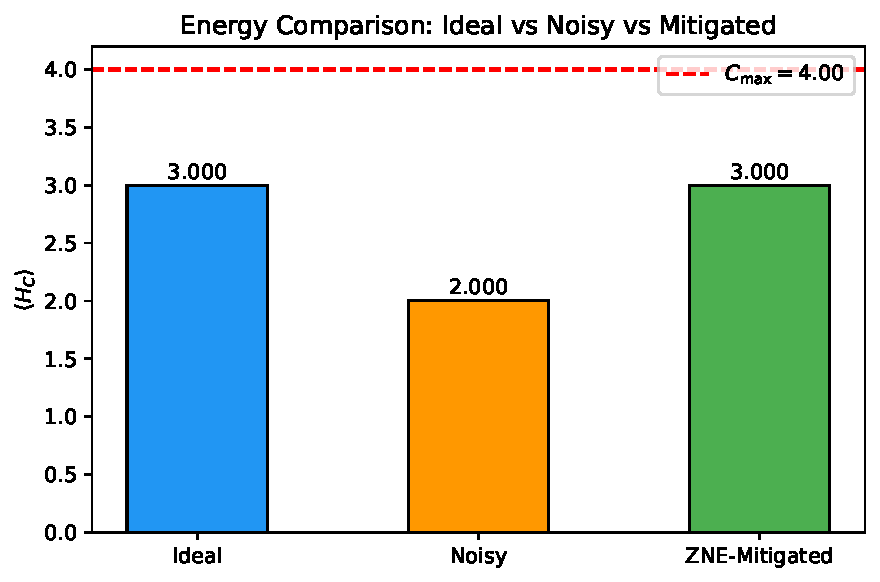
\includegraphics[width=0.75\textwidth]{report1_scripts/output/noise_comparison.pdf}
  \caption{Comparison of energy values: ideal ($E=3.0$), noisy ($E=2.0$), and
  ZNE-mitigated ($E=3.0$).  Zero-noise extrapolation successfully recovers the
  noiseless result.}
  \label{fig:noise-comparison}
\end{figure}

% ══════════════════════════════════════════════════════════════════════════════
\section{Conclusion}\label{sec:conclusion}

We have presented a complete, end-to-end mathematical walkthrough of the QAOA
Energy Landscape Explorer applied to the MaxCut problem on the 4-node cycle
graph $C_4$.  The pipeline consisted of:

\begin{enumerate}
  \item \textbf{Problem formulation}: Defining MaxCut on $C_4$ and encoding it
        as an Ising cost function (Section~\ref{sec:problem}).
  \item \textbf{Hamiltonian construction}: Deriving the diagonal cost
        Hamiltonian $H_C = 2I - \tfrac{1}{2}(Z_0Z_1 + Z_1Z_2 + Z_2Z_3 +
        Z_3Z_0)$ and verifying its eigenvalues against classical cut values
        (Section~\ref{sec:hamiltonian}).
  \item \textbf{Circuit construction}: Building the $p=1$ QAOA circuit with
        $\mathrm{IsingZZ}$ cost gates and $R_X$ mixer gates
        (Section~\ref{sec:circuit}).
  \item \textbf{Energy landscape}: Scanning the two-parameter landscape
        $E(\gamma,\beta)$, identifying its periodicity and symmetry, and
        locating the global optimum (Section~\ref{sec:landscape}).
  \item \textbf{Classical optimization}: Using COBYLA to find optimal
        parameters $\gamma^*\approx\pi/4$, $\beta^*\approx 5\pi/8$, achieving
        $E^*=3.0$ and approximation ratio $r=0.75$ in 43 evaluations
        (Section~\ref{sec:optimization}).
  \item \textbf{Noise and mitigation}: Simulating depolarizing and thermal
        relaxation noise ($E_{\text{noisy}}=2.0$) and recovering the noiseless
        result via ZNE ($E_{\text{ZNE}}=3.0$)
        (Section~\ref{sec:noise}).
\end{enumerate}

This worked example demonstrates that even at the shallowest circuit depth
($p=1$), QAOA produces a structured, smooth energy landscape with analytically
predictable optima, and that zero-noise extrapolation can effectively
counteract realistic hardware noise on small instances.

% ══════════════════════════════════════════════════════════════════════════════
\begin{thebibliography}{9}

\bibitem{farhi2014}
  E.~Farhi, J.~Goldstone, and S.~Gutmann,
  ``A Quantum Approximate Optimization Algorithm,''
  \emph{arXiv:1411.4028}, 2014.

\bibitem{wang2018}
  Z.~Wang, S.~Hadfield, Z.~Jiang, and E.~G.~Rieffel,
  ``Quantum Approximate Optimization Algorithm for MaxCut: A Fermionic View,''
  \emph{Phys.\ Rev.\ A}, vol.~97, p.~022304, 2018.

\bibitem{powell1994}
  M.~J.~D.~Powell,
  ``A direct search optimization method that models the objective and
  constraint functions by linear interpolation,''
  in \emph{Advances in Optimization and Numerical Analysis}, pp.~51--67, 1994.

\bibitem{temme2017}
  K.~Temme, S.~Bravyi, and J.~M.~Gambetta,
  ``Error mitigation for short-depth quantum circuits,''
  \emph{Phys.\ Rev.\ Lett.}, vol.~119, p.~180509, 2017.

\bibitem{li2017}
  Y.~Li and S.~C.~Benjamin,
  ``Efficient variational quantum simulator incorporating active error
  minimization,''
  \emph{Phys.\ Rev.\ X}, vol.~7, p.~021050, 2017.

\end{thebibliography}

\end{document}
